% Epistatic Circuits — NEMI 2026 poster, v1
% tikzposter 3x3 block format, matching grokking_poster_v2.tex.
%
%   lualatex epistasis_poster_v1.tex

\documentclass[25pt, a0paper, portrait]{tikzposter}

\usepackage{amsmath,amssymb}
\usepackage{booktabs}
\usepackage{graphicx}
\usepackage{enumitem}
\usepackage{microtype}

\graphicspath{{../paper/figures/}}

% ── Color palette ───────────────────────────────────────
\definecolor{sub}{HTML}{2980B9}
\definecolor{super}{HTML}{E74C3C}
\definecolor{additive}{HTML}{95A5A6}
\definecolor{epiorange}{HTML}{FF9800}
\definecolor{darktext}{HTML}{2C3E50}
\definecolor{blockbg}{HTML}{FFFFFF}

% ── Theme ───────────────────────────────────────────────
\usetheme{Default}

\definecolorstyle{EpiColors}{
  \definecolor{colorOne}{HTML}{2C3E50}
  \definecolor{colorTwo}{HTML}{3498DB}
  \definecolor{colorThree}{HTML}{ECF0F1}
}{
  \colorlet{backgroundcolor}{colorThree}
  \colorlet{framecolor}{colorOne}
  \colorlet{titlefgcolor}{white}
  \colorlet{titlebgcolor}{colorOne}
  \colorlet{blocktitlebgcolor}{colorTwo}
  \colorlet{blocktitlefgcolor}{white}
  \colorlet{blockbodybgcolor}{blockbg}
  \colorlet{blockbodyfgcolor}{darktext}
  \colorlet{notefgcolor}{darktext}
  \colorlet{notebgcolor}{epiorange!15}
  \colorlet{notefrcolor}{epiorange}
}
\usecolorstyle{EpiColors}

\defineblockstyle{EpiBlock}{
  titlewidthscale=1.0, bodywidthscale=1.0, titleleft,
  titleoffsetx=0pt, titleoffsety=0pt,
  bodyoffsetx=0pt, bodyoffsety=0pt, bodyverticalshift=0pt,
  roundedcorners=12, linewidth=2pt, titleinnersep=10pt, bodyinnersep=15pt
}{
  \draw[rounded corners=\blockroundedcorners, color=blocktitlebgcolor,
        fill=blockbodybgcolor, line width=\blocklinewidth]
    (blockbody.south west) rectangle (blocktitle.north east);
  \ifBlockHasTitle
    \draw[rounded corners=\blockroundedcorners,
          fill=blocktitlebgcolor, color=blocktitlebgcolor,
          line width=\blocklinewidth]
      (blocktitle.south west) rectangle (blocktitle.north east);
  \fi
}
\useblockstyle{EpiBlock}

\definetitlestyle{EpiTitle}{
  width=\paperwidth, roundedcorners=0, linewidth=0pt, innersep=20pt,
  titletotopverticalspace=15mm, titletoblockverticalspace=25mm
}{
  \draw[fill=titlebgcolor, color=titlebgcolor]
    (\titleposleft, \titleposbottom)
    rectangle (\titleposright, \titlepostop);
}
\usetitlestyle{EpiTitle}

\title{%
  \parbox{0.92\linewidth}{\centering\bfseries
    Epistatic Circuits\\[6pt]
    Walsh--Hadamard Interaction Decomposition\\[3pt]
    for Neural Network Mechanisms}}
\author{Elliot Tower\quad\texttt{elliot@elliottower.ai}}
\institute{}

\begin{document}

\maketitle[width=\paperwidth]

% ════════════════════════════════════════════════════════
% ROW 1
% ════════════════════════════════════════════════════════
\begin{columns}
\column{0.33}

\block{The Problem}{
  Circuit discovery methods decompose neural networks into subgraphs
  that explain a behavior. Every method in current use is
  \textbf{additive by construction}: it scores each component
  independently and assembles a circuit from the top-scoring set.

  \vspace{6mm}
  Transformers are structurally non-additive. Components interact:
  removing one changes what another does. Additive methods cannot
  detect, measure, or preserve this interaction structure.

  \vspace{6mm}
  \textbf{The question:} what is the exact pairwise interaction
  structure of a circuit, what do existing methods retain of it,
  and does the discarded structure carry mechanism?
}

\column{0.34}

\block{The Walsh--Hadamard Decomposition}{
  A coalition sweep over $n$ heads evaluates all $2^n$ subsets. The
  Walsh--Hadamard transform decomposes the resulting function into
  exact interaction orders:

  \vspace{4mm}
  \begin{itemize}[leftmargin=*, itemsep=3mm]
    \item \textbf{Order 1:} individual head effects
    \item \textbf{Order 2:} pairwise interactions $w_{ij}$
    \item \textbf{Order 3+:} higher-order terms
  \end{itemize}

  \vspace{4mm}
  Each coefficient $w_{ij}$ is the exact deviation from additivity
  for heads $i$ and $j$, with no regularization and no held-out set.

  \vspace{4mm}
  \textcolor{sub}{\textbf{Sub-additive}} $\to$ shared pathway\\
  \textcolor{additive}{\textbf{Near-zero}} $\to$ independent\\
  \textcolor{super}{\textbf{Super-additive}} $\to$ mutual compensation
}

\column{0.33}

\block{Compressed Sensing Makes It Scale}{
  Brute-force cost: $2^n$ forward passes. For $n{=}20$ heads, that
  is ${\sim}10^6$ evaluations.

  \vspace{4mm}
  \textbf{The interaction spectrum is sparse.} LASSO recovery from
  $M$ random coalitions reaches the exact spectrum:

  \vspace{4mm}
  \begin{center}
  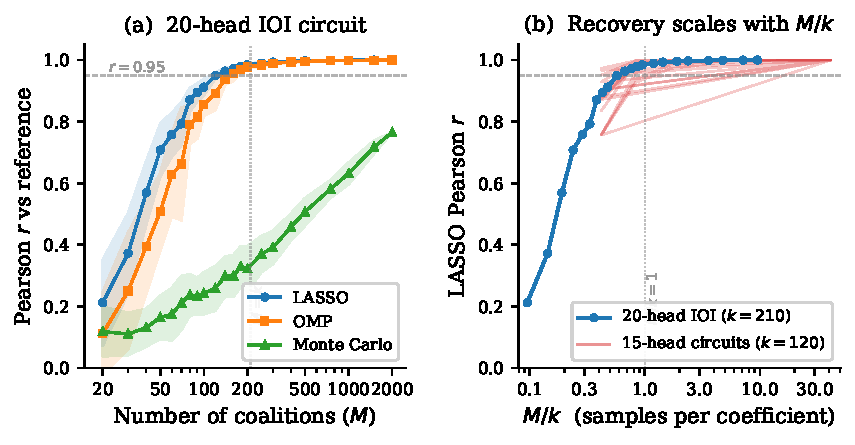
\includegraphics[width=0.95\linewidth]{sparse_walsh_recovery.pdf}
  \end{center}

  \vspace{2mm}
  Correlation $r > 0.95$ at $M = 140$ for a 20-head circuit.
  \textbf{7{,}490$\times$ compression} over exact enumeration.

  \vspace{4mm}
  Theoretical brackets: generic RIP bound gives $M \approx 1{,}400$;
  structured Walsh bound gives $M \approx 13{,}000$. Recovery
  succeeds well below both.
}

\end{columns}

% ════════════════════════════════════════════════════════
% ROW 2
% ════════════════════════════════════════════════════════
\begin{columns}
\column{0.33}

\block{Selective Pressures Across Methods}{
  Three families of circuit proxies, audited against Walsh ground truth:

  \vspace{4mm}
  \begin{center}
  \begin{tabular}{lc}
    \toprule
    \textbf{Proxy family} & \textbf{Agreement} \\
    \midrule
    Weight geometry & $R^2 < 0$ (all 30) \\
    EAP edge attribution & $\rho = 0.58$ \\
    Path patching & $r = 0.07$ \\
    \bottomrule
  \end{tabular}
  \end{center}

  \vspace{4mm}
  \textbf{Weight geometry predicts nothing.} Composition scores and
  subspace overlap carry zero cross-validated power for pairwise
  interaction under any ablation primitive.

  \vspace{4mm}
  \textbf{EAP captures the linear component} while missing nonlinear
  routing effects.

  \vspace{4mm}
  \textbf{Path patching is orthogonal.} It measures direct causal
  edges; Walsh measures functional coupling. These are categorically
  different quantities.

  \vspace{3mm}
  \begin{center}
  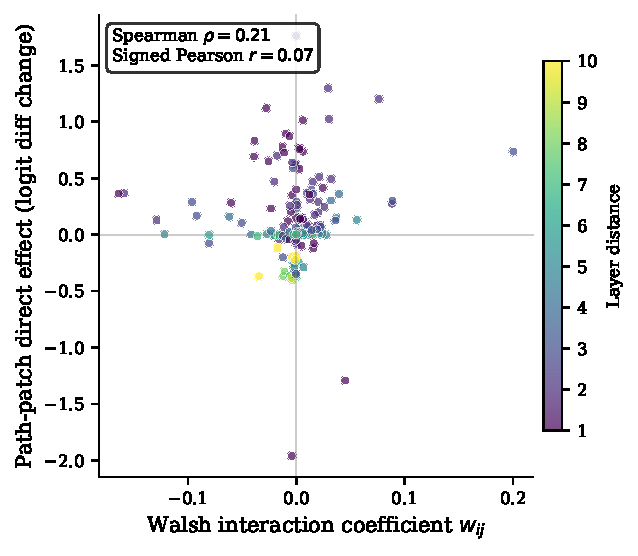
\includegraphics[width=0.95\linewidth]{path_patching_scatter.pdf}
  \end{center}
}

\column{0.34}

\block{The Complementation Test}{
  Genetics decides whether two mutations belong to one functional unit
  using Benzer's cis-trans test. The Walsh interaction matrix provides
  exactly this data for every head pair.

  \vspace{4mm}
  Hierarchical clustering on the signed masking matrix for the 15-head
  IOI circuit, with cluster count selected by silhouette:

  \vspace{4mm}
  \begin{center}
  \begin{tabular}{lc}
    \toprule
    \textbf{Result} & \\
    \midrule
    ARI vs.\ published taxonomy & $+0.571$ \\
    ARI vs.\ raw layer depth    & $+0.053$ \\
    Bootstrap merge rate (S-inh.\ $\sim$ neg.\ NM) & 1000/1000 \\
    \bottomrule
  \end{tabular}
  \end{center}

  \vspace{4mm}
  S-inhibition heads and negative name movers merge into
  \textbf{one functional unit} in every bootstrap resample, every
  ablation type, and every linkage method.

  \vspace{4mm}
  The merge is asymmetric: S-inhibition merges with negative name
  movers (4/4 conditions) but separates from name movers (0/2).
  The OV sign difference explains this --- negative heads
  \textbf{invert} rather than diminish, so removing S-inhibition
  redirects their write from $-\mathrm{IO}$ to $+\mathrm{IO}$.

  \vspace{3mm}
  \begin{center}
  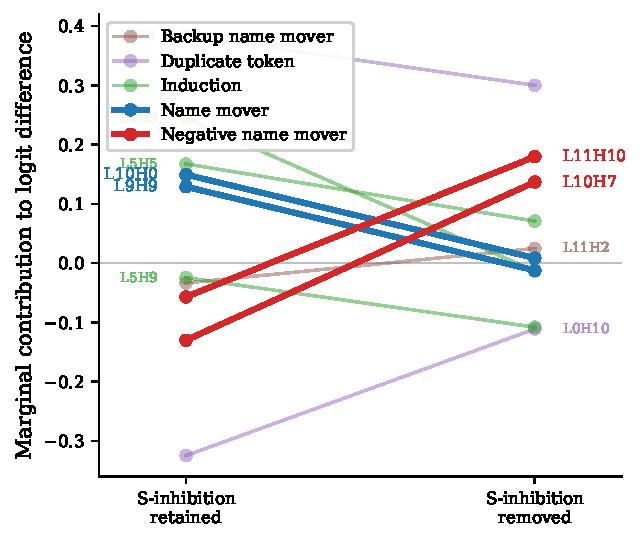
\includegraphics[width=0.95\linewidth]{conditional_marginal.pdf}
  \end{center}
}

\column{0.33}

\block{Energy Spectrum Across Six Tasks}{
  60 sweeps across six tasks in GPT-2 small. Energy fractions averaged
  over real (non-random) circuits within each task.

  \vspace{4mm}
  {\small
  \begin{tabular}{lccc}
    \toprule
    \textbf{Task} & \textbf{Ord-1} & \textbf{Ord-2} & \textbf{Ord-3+} \\
    \midrule
    IOI              & 0.82 & \textbf{0.15} & 0.03 \\
    RTI              & 0.81 & \textbf{0.13} & 0.06 \\
    Greater-than     & 0.92 & 0.07 & 0.01 \\
    Induction        & 0.90 & 0.08 & 0.02 \\
    SVA              & 0.95 & 0.05 & 0.00 \\
    Gendered pronoun & 0.99 & 0.01 & 0.00 \\
    \midrule
    Random           & 0.92 & 0.06 & 0.02 \\
    \bottomrule
  \end{tabular}
  }

  \vspace{4mm}
  IOI and RTI circuits carry 13--15\% pairwise interaction energy.
  Gendered pronoun circuits carry ${\sim}1\%$. The variation reflects
  task structure: coordinated attention routing versus independently
  operating heads.

  \vspace{4mm}
  Order-3+ energy rarely exceeds 5\%. \textbf{Interactions are
  predominantly pairwise.}

  \vspace{3mm}
  \begin{center}
  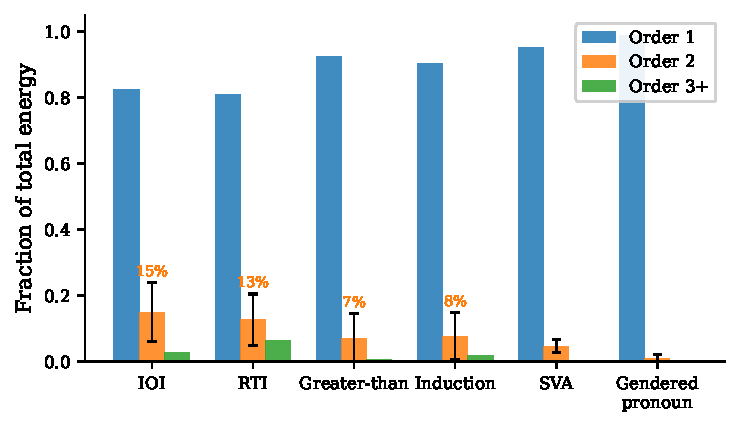
\includegraphics[width=0.95\linewidth]{energy_spectrum.pdf}
  \end{center}
}

\end{columns}

% ════════════════════════════════════════════════════════
% ROW 3
% ════════════════════════════════════════════════════════
\begin{columns}
\column{0.33}

\block{MIB Benchmark}{
  Walsh-based circuit discovery on the MIB faithfulness benchmark:

  \vspace{4mm}
  \begin{center}
  \begin{tabular}{lc}
    \toprule
    \textbf{Method} & \textbf{CPR} \\
    \midrule
    Walsh (order-1) & \textbf{0.996} \\
    Activation patching & 0.937 \\
    EAP-IG & 0.917 \\
    ACDC & 0.895 \\
    \bottomrule
  \end{tabular}
  \end{center}

  \vspace{3mm}
  \begin{center}
  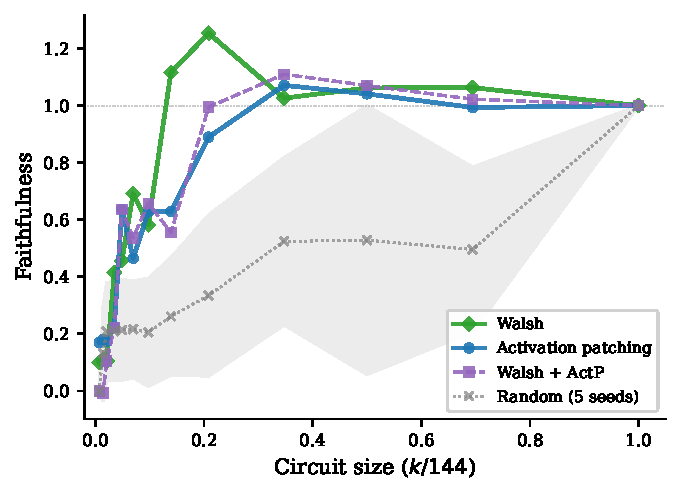
\includegraphics[width=0.95\linewidth]{mib_faithfulness_curves.pdf}
  \end{center}

  \vspace{2mm}
  Walsh order-1 coefficients, computed as a byproduct of the
  interaction decomposition, outperform dedicated circuit discovery
  methods on faithfulness at all circuit sizes.
}

\column{0.34}

\block{What the Discarded Structure Carries}{
  Additive circuit summaries discard the order-2 spectrum entirely.
  For the IOI circuit, that spectrum carries:

  \vspace{5mm}
  \begin{itemize}[leftmargin=*, itemsep=4mm]
    \item A \textbf{sign-inversion dependency} between S-inhibition
      and negative name movers that the original analysis recorded
      as unexplained
    \item A \textbf{functional unit boundary} that separates two head
      classes with identical input structure by OV sign
    \item A \textbf{masking hierarchy} where S-inhibition gates the
      function of every downstream head class
    \item The \textbf{super-additive} interaction ($1.9\times$) at the
      module level that makes backup name movers effective
  \end{itemize}

  \vspace{5mm}
  None of this is visible from individual head scores. It exists
  in the relations between heads, which is where the Walsh spectrum
  lives.
}

\column{0.33}

\block{Takeaway}{
  \textbf{The pairwise interaction structure of a neural network
  circuit is measurable, compressible, and carries mechanism that
  additive circuit summaries discard.}

  \vspace{6mm}
  \begin{itemize}[leftmargin=*, itemsep=4mm]
    \item Walsh--Hadamard decomposition gives exact ground truth
    \item Compressed sensing: $r > 0.95$ from 140 coalitions
      ($7{,}490\times$ compression)
    \item Weight geometry predicts nothing; path patching is
      orthogonal; EAP captures linear coupling
    \item The complementation test recovers the S-inhibition /
      negative name-mover dependency
  \end{itemize}

  \vspace{8mm}
  \begin{center}
  \texttt{elliot@elliottower.ai}

  \vspace{3mm}
  {\small 4 pre-registrations with SHA commitments.}

  \vspace{2mm}
  {\small Code, data, and pre-registrations:}

  \texttt{github.com/elliottower/epistatic-circuits}
  \end{center}
}

\end{columns}

\end{document}
